\documentclass[11pt, oneside]{article}      % use "amsart" instead of "article" for AMSLaTeX format
\usepackage{ZX-Jones_preamble}
\usepackage{ZX-Jones_definitions}

\title{\textbf{Efficiently Calculating Jones Polynomials at Lattice Roots of Unity with the ZX-Calculus (Draft)}}
\author{
  Alex Townsend-Teague
  \and
  Konstantinos Meichandzitis
}
\date{}

\begin{document}
\maketitle

\section{Introduction}

[Use Konstantinos' O.G. notes from the start of this project, and introduce the qubit and qutrit ZX calculi]\newline

For the case $q=3$ we use the qutrit ZX calculus:
\begin{equation}
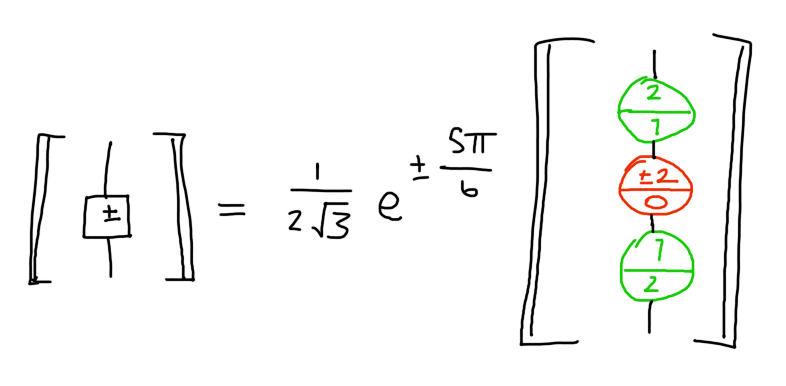
\includegraphics[scale=0.3]{figures/sketches/Qutrit Potts matrices.png}
\end{equation}

For the case $q=4$ we are back again in the usual qubit ZX calculus:
\begin{equation}
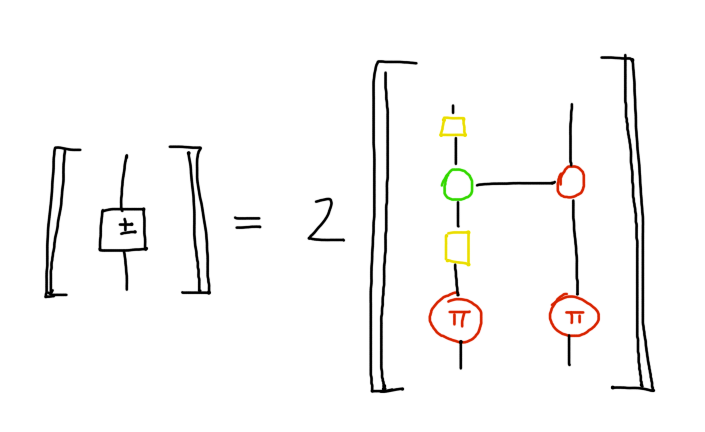
\includegraphics[scale=0.3]{figures/sketches/Qu(4)it Potts matrices.png}
\end{equation}

In each case, the resulting map is in the stabilizer fragment of the ZX calculus. 

\section{Simplifying Qubit ZX Diagrams}

In [cite Aleks' paper] the authors give an efficient algorithm for reducing any qubit stabilizer ZX diagram to one of vastly smaller size [specific bound?]. In our case, since any knot will be transformed by the process above into a ZX diagram with zero inputs and zero outputs, this gives an efficient algorithm for reducing the diagram to a scalar.\newline

[Summarise Aleks' algorithm]\newline

This suffices to prove our main result for the cases $q \in \{2, 4\}$. However, it doesn't yet give us a useful algorithm for explicitly calculating Jones polynomials, because throughout the method above equality is considered only up to a complex scalar multiple. Therefore we now give a scalar-exact version.\newline

[Give scalar-exact version]\newline

\section{Simplifying Qutrit ZX Diagrams}

For the remaining case $q=3$, we will show that we can generalise all the ideas of the previous section to the qutrit ZX calculus.

\subsection{Graph-Like Qutrit ZX Diagrams}

% \numbered{Definition}{A \textit{Hadamard edge} (or \textit{H-edge}) is a Hadamard map connecting two spiders. A \textit{Hadamard adjoint edge} (or \textit{$H^\dagger$-edge) }}

[Make all of the following scalar-exact]\newline

We first define a graph-like diagram in the qutrit ZX calculus.

% \numbered{Definition}{A qutrit ZX diagram is \textit{graph-like} when:}
\begin{definition}\label{def:graph_like_qutrit}
A qutrit ZX diagram is \textit{graph-like} when: 
\begin{enumerate}
	\item Every spider is a Z-spider.
	\item Spiders are only connected by Hadamard edges ($H$-edges) or their adjoints ($H^\dagger$-edges).
	\item Every pair of spiders is connected by at most one $H$-edge or $H^\dagger$-edge.
	\item Every input and output is connected to a spider.
	\item Every spider is connected to at most one input or output.
\end{enumerate}
\end{definition}

For our specific needs, the last two items above will not be relevant, since ZX-diagrams arising from knots will have no inputs or outputs, but we include them to keep the definition consistent with the qubit case. However, note the difference compared to the qubit case: we need not worry about self-loops beacuse the qutrit ZX calculus doesn't define a `plain' cap or cup. But this comes at a cost: spiders in the qutrit case fuse more fussily. Specifically, when two spiders of the same colour are connected by at least one plain edge and at least one $H$- or $H^\dagger$-edge, fusion is not possible. The following equation, which holds with the roles of $H$ and $H^\dagger$ reversed, helps us get around this:

\begin{equation}\label{eq:spiders_reluctant_to_fuse}
	\tikzfig{spiders_reluctant_to_fuse} 
\end{equation}

We will shortly show that every qutrit ZX diagram is equivalent to a graph-like one, making use of the following lemmas:

\begin{lemma}\label{lem:H_edges_qutrit} 
	The following two equations hold in the qutrit ZX calculus. Moreover, they hold with the roles of $H$ and $H^\dagger$ interchanged:
	\begin{equation}
		\tikzfig{2_hadamard_edges_become_adjoint}
		\hspace{75pt}
		\tikzfig{hadamard_edge_and_adjoint_edge_permute}
	\end{equation}
	\begin{proof}
		This is Lemma 3.4 in [cite Harny's local complementation paper].
	\end{proof}
\end{lemma}

As we will formalise later, the lemma above says we can think of Hadamard edges as $1$-weighted edges and their adjoints as $2$-weighted edges, then work modulo $3$, since every triple of parallel edges disappears. This motivates defining `parametrised' Hadamard gates, which will come in use later:

\begin{equation}
	\tikzfig{parametrised_hadamard_1}
	\hspace{75pt}
	\tikzfig{parametrised_hadamard_2}
\end{equation}

Where the previous lemma relates single $H$- and $H$-boxes across multiple edges, the next relates multiple $H$- and $H^\dagger$- boxes on single edges.

\begin{lemma}\label{lem:H_boxes_qutrit} 
	The following three equations hold in the qutrit ZX calculus. Moreover, they hold with the roles of $H$ and $H^\dagger$ interchanged:
	\begin{equation}
		\tikzfig{4_hadamards_cancel}
		\hspace{75pt}
		\tikzfig{3_hadamards_flip}
		\hspace{75pt}
		\tikzfig{2_hadamards_separate}
	\end{equation}
	\begin{proof}
	\end{proof}
\end{lemma}

Again intuitively we can think of Hadamard boxes of having value $1$ and their adjoints $-1$ and then work modulo $4$.

\begin{corollary}\label{prop:every_diagram_is_graph_like_qutrit}
	Every qutrit ZX diagram is equivalent to one that is graph-like.
	\begin{proof}
		First use the colour change rule to turn all X-spiders into Z-spiders. Then use Lemma~\ref{lem:H_boxes_qutrit} to remove excess $H$- and $H^\dagger$-boxes, inserting a spider between any remaining consecutive pair of such boxes, so that all spiders are connected only by plain edges, $H$-edges or $H^\dagger$-edges. Fuse together as many as possible, and apply Equation~\ref{eq:spiders_reluctant_to_fuse} where fusion is not possible, so that no plain edge connects two spiders. Apply Lemma~\ref{lem:H_edges_qutrit} to all connected pairs of spiders until at most one $H$- or $H^\dagger$-edge remains between them. Finally, to ensure every input and output is connected to a spider and every spider is connected to at most one input or output, we can again add a few spiders, $H$- and $H^\dagger$-boxes as needed: 
		\begin{equation}
			\tikzfig{plain_input_output_wire_is_graph-like}
			\hspace{75pt}
			\tikzfig{input_connected_to_hadamard_is_graph-like}
			\hspace{75pt}
			\tikzfig{multiple_inputs_connected_to_one_spider_is_graph-like}
		\end{equation}
	\end{proof}
\end{corollary}

\begin{definition}\label{def:graph_state_qutrit}
	A graph-like qutrit ZX diagram is a \textit{graph state} when every spider has zero phase (top and bottom) and is connected to an output. 
\end{definition}

A graph state is described fully by its underlying multigraph, or equivalently by an adjacency matrix, where edges take weights in $\mathbb{Z}_3$ [reference Harny]. Nodes correspond to phaseless green spiders, edges of weight $1$ correspond to Hadamard edges, and edges of weight $2$ correspond to $H^\dagger$ edges. As in the qubit case, graph states admit a local complementation operation [Harny's completeness paper, Definition 2.6], though the effect is now slightly more complicated. We'll give the intuition after the formal definition:

\begin{definition}\label{def:local_complementation_qutrit}
	Given $a \in \mathbb{Z}_3$ and a graph state $G$ with adjacency matrix $W = (w_{i,j})$, the \textit{$a$-local complentation} at node $k$ is the new graph state $G *_a i$, whose adjacency matrix $W' = (w'_{i,j})$ given by:
	\begin{equation}
		w'_{i,j} = w_{i,j} + aw_{i,k}w_{j,k}
	\end{equation}
\end{definition}

So only those edges between neighbours of node $k$ are affected, but rather than just having their weight increased by $1$ (modulo $2$) as in the qubit case, the increase in weight also depends on the weights of the edges from $i$ and $j$ to $k$. As always, this is best seen graphically. We reintroduce the blue dashed line notation for Hadamard edges, and now also use purple dashed lines for $H^\dagger$-edges:

\begin{equation}
	\tikzfig{blue_dashed_line_definition}
	\hspace{75pt}
	\tikzfig{purple_dashed_line_definition}
\end{equation} 

So now for two nodes $i$ and $j$ both connected to $k$ by the same colour edge, $a$-local complementation at $k$ increases weight $w_{i,j}$ by $a$. If instead $i$ and $j$ are connected to $k$ by edges of different colour, $a$-local complementation at $k$ decreases $w_{i,j}$ by $a$. We show a fragment of a ZX-diagram below under the effect of this operation:

\begin{equation}
	\tikzfig{a_local_comp_same}
	\hspace{75pt}
	\tikzfig{a_local_comp_different}
\end{equation}

But the fragment above doesn't give the full picture. As in the qubit case, local complementation gives an equality up to introducing some single qubit phase gates on the outputs.

\begin{theorem}\label{thm:local_comp_equality}
	Given $a \in \mathbb{Z}_3$ and a graph state $(G, W)$ containing a node $k$, let $N(k)$ denote the neighbours of $k$ - that is, nodes $i$ with weight $w_{i,k} \in \{1, 2\}$. Then the following equality holds:
	\ctikzfig{local_comp_on_graph_state}
	\begin{proof}
		This is Theorem 4.4 and Corollary 4.5 in [Harny's completeness paper]
	\end{proof}
\end{theorem}

Composing local complementations gives a local pivot operation.

\begin{definition}\label{def:local_pivot_qutrit}
	Given $a,b,c \in \mathbb{Z}_3$ and a graph state $G$ containing nodes $i$ and $j$, the \textit{$(a,b,c)$-local pivot} along $ij$ is the new graph state $G \wedge_{(a,b,c)} ij \defeq ((G *_a i) *_b j) *_c i$. 
\end{definition}

This again results in an equality, up to introducing some extra gates on outputs. Here we shall only consider an $(a,-a,a)$-local pivot along an edge $ij$ of non-zero weight, for $a \in \{1, 2\}$. We will call this a \textit{proper $a$-local pivot} along $ij$, and denote it $G \wedge_a ij$.

\begin{theorem}\label{thm:local_pivot_equality}
	Given $a \in \mathbb{Z}_3$ and a graph state $(G, W)$ containing connected nodes $i$ and $j$, define the following:
	\begin{itemize}
		\item $N_{=}(i, j) \defeq \left\{k \in N(i) \cap N(j) \mid w_{k,i} = w_{k,j} \right\}$
		\item $N_{\neq}(i, j) \defeq \left\{k \in N(i) \cap N(j) \mid w_{k,i} \neq w_{k,j} \right\}$
	\end{itemize} 
	Then the following equation relates $G$ and its proper $a$-local pivot along $ij$:
	\ctikzfig{proper_local_pivot_on_graph_state}
\end{theorem}

These two operations are again the drivers behind the simplification procedure. We classify spiders into three families:

\begin{equation}
	\mathcal{M} = \left\{\qutritZspider{1}{2}, \qutritZspider{2}{1}\right\},
	\hspace{10pt}
	\mathcal{N} = \left\{\qutritZspider{0}{1}, \qutritZspider{1}{0}, \qutritZspider{0}{2}, \qutritZspider{2}{0}\right\},
	\hspace{10pt}
	\mathcal{P} = \left\{\qutritZspider{1}{1}, \qutritZspider{2}{2}\right\}.
\end{equation}

 This is as seen in~\cite[][Theorem 3.1]{harny_completeness} except here we don't class the zero-phase spider as an \Mspider. We call a spider in a graph-like ZX-diagram \textit{interior} if it isn't connected to an input or output. Thus for our use case all spiders are interior. Given any graph-like ZX-diagram, we will show that we can eliminate pairs of connected interior \Mspiders\ by local pivoting, and standalone interior $\mathcal{N}$- and \Pspiders\ by local complementation.\newline

\begin{theorem}\label{thm:eliminate_M_spiders}
	Given any graph-like ZX-diagram containing two interior \Mspiders\ $i$ and $j$ connected by edge $ij$ of weight $w_{i,j} \eqdef w \in \{1,2\}$, suppose we perform a proper $\pm w$-local pivot along $ij$. Then the new ZX-diagram is related to the old one by the equality:
	
	\ctikzfig{eliminate_M_spiders/theorem_LHS}
	\ctikzfig{eliminate_M_spiders/theorem_RHS}
	
	where all changes to weights of edges where neither endpoint is $i$ or $j$ are omitted. Furthermore, in order to save space, each node with phase \qutritZphase{a_x^y}{b_x^y} is representative of \textit{all} nodes connected to $i$ by an $x$-weighted edge and to $j$ by a $y$-weighted edge.
\end{theorem}

\begin{theorem}\label{thm:eliminate_N_spiders}
	Given any graph-like ZX-diagram containing an interior \Nspider\ $k$ with phase \qutritZphase{0}{n} for $n \in \{1,2\}$, suppose we perform a $(-n)$-local complementation at $k$. Then the new ZX-diagram is related to the old one by the equality:

	\begin{equation*}
		\tikzfig{eliminate_N_spiders/0_n/step_1} \quad = \quad \tikzfig{eliminate_N_spiders/0_n/step_9}
	\end{equation*}

	where all changes to weights of edges where neither endpoint is $k$ are omitted. If instead $k$ has phase \qutritZphase{n}{0} for $n \in \{1,2\}$, suppose we perform the same $(-n)$-local complementation at $k$. Then the equality relating the new and old diagrams becomes:

	% Spiders with phases \qutritZphase{a_1}{b_1} ... \qutritZphase{a_r}{b_r} are all the neighbours of $k$ connected by a $1$-weighted (blue) edge, while spider with phases \qutritZphase{c_1}{d_1} ... \qutritZphase{c_s}{d_s} are all the neighbours of $k$ connected by a $2$-weighted (purple) edge.\newline

	\begin{equation*}
		\tikzfig{eliminate_N_spiders/n_0/step_1} \quad = \quad \tikzfig{eliminate_N_spiders/n_0/step_9}
	\end{equation*}
\end{theorem}

\begin{theorem}\label{thm:eliminate_P_spiders}
	Given any graph-like ZX-diagram containing an interior \Pspider\ $k$ with phase \qutritZphase{p}{p} for $p \in \{1,2\}$, suppose we perform a $p$-local complementation at $k$. Then the new ZX-diagram is related to the old one by the equality:

	\begin{equation*}
		\tikzfig{eliminate_P_spiders/step_1} \quad = \quad \tikzfig{eliminate_P_spiders/step_9}
	\end{equation*}

	where all changes to weights of edges where neither endpoint is $k$ are omitted. 

	% Spiders with phases \qutritZphase{a_1}{b_1} ... \qutritZphase{a_r}{b_r} are all the neighbours of $k$ connected by a $1$-weighted (blue) edge, while spider with phases \qutritZphase{c_1}{d_1} ... \qutritZphase{c_s}{d_s} are all the neighbours of $k$ connected by a $2$-weighted (purple) edge.\newline
\end{theorem}

We can now combine these three elimination theorems into an algorithm for efficiently simplifying a graph-like ZX-diagram with no inputs or outputs. First note that after applying any one of the three elimination theorems to such a diagram we may end up with a state that is no longer graph-like. Fortunately the only way in which this can happen is if two spiders end up being connected by multiple $H$- or $H^\dagger$-edges, and we have shown in Lemma~\ref{lem:H_edges_qutrit} that these can always be reduced to just one edge.

\begin{theorem}\label{thm:simplification_algorithm_works}
	Given any graph-like ZX-diagram with no inputs or outputs, the following algorithm will always terminate after a finite number of steps, returning an equivalent graph-like ZX-diagram with no \Nspiders, \Pspiders, or adjacent pairs of \Mspiders. Repeat the steps below until no rule matches. After each step, apply Lemma~\ref{lem:H_edges_qutrit} as needed until the resulting diagram is graph-like:
	\begin{enumerate}
		\item Eliminate an \Nspider\ via Theorem~\ref{thm:eliminate_N_spiders}.
		\item Eliminate a \Pspider\ via Theorem~\ref{thm:eliminate_P_spiders}.
		\item Eliminate two adjacent \Mspiders\ via Theorem~\ref{thm:eliminate_M_spiders}.
	\end{enumerate}
	\begin{proof}
		At every step the total number of spiders decreases by at least one, so since we start with a finite diagram the algorithm terminates after a finite number of steps. By construction, when it does so we are left with an equivalent graph-like ZX-diagram with no \Nspiders, \Pspiders, or adjacent pairs of \Mspiders.
	\end{proof}
\end{theorem}

\begin{corollary}\label{cor:stabilizer_simplification_algorithm_works}
	In particular, if we start with a stabilizer diagram, we can eliminate all but perhaps $1$ \Mspider, depending on whether the initial number of \Mspiders\ was odd or even. 
	\begin{proof}
		No step introduces any non-stabilizer phases.
	\end{proof}
\end{corollary}

The algorithm above could be extended to graph-like diagrams with inputs or outputs as in the qubit case, but since for our purposes we don't need to do so, we have not gone to the trouble.

\bibliography{ZX-Jones}

\section{Appendix}

We begin with a proof of the local pivot equality from Theorem~\ref{thm:local_pivot_equality}.\newline

\textbf{Theorem~\ref{thm:local_pivot_equality}.}
	Given $a \in \mathbb{Z}_3$ and a graph state $(G, W)$ containing connected nodes $i$ and $j$, define the following:
	\begin{itemize}
		\item $N_{=}(i, j) \defeq \left\{k \in N(i) \cap N(j) \mid w_{k,i} = w_{k,j} \right\}$
		\item $N_{\neq}(i, j) \defeq \left\{k \in N(i) \cap N(j) \mid w_{k,i} \neq w_{k,j} \right\}$
	\end{itemize} 
	Then the following equation relates $G$ and its proper $a$-local pivot along $ij$:
	\ctikzfig{proper_local_pivot_on_graph_state}
	\begin{proof}
		Annoyingly, proving this in full generality in one go - i.e. for a proper $a$-local pivot along an edge $ij$ of weight $b$ - becomes a bit tricky diagramatically, because it becomes hard to keep track of all the variable edge weights. Fortunately the four cases ($a, b \in \{1,2\}$) split into two pairs of symmetric cases: $a = b$ and $a \neq b$.\newline

		Now, it suffices to only draw a fragment of a graph state. Certainly we consider nodes $i$ and $j$ and the edge $ij$ between them. Then define $N_x^y$ to be the set $\left\{k \mid w_{k,i} = x, w_{k,j} = y \right\}$, for $x, y, \in \mathbb{Z}_3$. We will consider a representative node $k_x^y$ from each $N_x^y \neq N_0^0$, as well as its edges $ik_x^y$ and $jk_x^y$. All other nodes and edges are irrelevant; this is because we are only interested in nodes and edges that \textit{affect} the three local complementation operations on $i$ and $j$ - we aren't concerned with those that are only \textit{affected by} the operations.\newline

		So for the case $a=b$, we show the proper $1$-local pivot along $ij$ of weight $1$:

		\begingroup
			\allowdisplaybreaks
			\setlength{\jot}{20pt}
			\begin{align*}
				&\ &&\tikzfig{proper_1_local_pivot/weight_1/step_1} &&&= &&&&\tikzfig{proper_1_local_pivot/weight_1/step_2} \\
				&= &&\tikzfig{proper_1_local_pivot/weight_1/step_3} &&&= &&&&\tikzfig{proper_1_local_pivot/weight_1/step_4} \\
				&= &&\tikzfig{proper_1_local_pivot/weight_1/step_5} &&&= &&&&\tikzfig{proper_1_local_pivot/weight_1/step_6} \\
			\end{align*}
		\endgroup

		The story is similar for the case $a \neq b$; here we show the proper $1$-local pivot along $ij$ of weight $2$:

		\begingroup
			\allowdisplaybreaks
			\setlength{\jot}{20pt}
			\begin{align*}
				&\ &&\tikzfig{proper_1_local_pivot/weight_2/step_1} &&&= &&&&\tikzfig{proper_1_local_pivot/weight_2/step_2} \\
				&= &&\tikzfig{proper_1_local_pivot/weight_2/step_3} &&&= &&&&\tikzfig{proper_1_local_pivot/weight_2/step_4} \\
				&= &&\tikzfig{proper_1_local_pivot/weight_2/step_5} &&&= &&&&\tikzfig{proper_1_local_pivot/weight_2/step_6} \\
			\end{align*}
		\endgroup

		% \ctikzfig{proper_1_local_pivot_weight_2_line_1}
		% \ctikzfig{proper_1_local_pivot_weight_2_line_2}
		% \ctikzfig{proper_1_local_pivot_weight_2_line_3}

		The case $a=b=2$ is the same as $a=b=1$, except with the roles of purple and blue edges interchanged, so by symmetry of the diagram the only difference is in the phase gates added to the outputs. Namely, on each phase gate we replace all instances of $1$ with a $2$. Thus the roles of $H$ and $H^\dagger$ are swapped too. Likewise for the case $(a,b) = (2,1)$ with respect to the case $(a,b) = (1,2)$.

	\end{proof}

Here we prove the three elimination theorems for $\mathcal{M}$-, $\mathcal{N}$- and \Pspiders.

\textbf{Theorem~\ref{thm:eliminate_M_spiders}.}
	Given any graph-like ZX-diagram containing two interior \Mspiders\ $i$ and $j$ connected by edge $ij$ of weight $w_{i,j} \eqdef w \in \{1,2\}$, suppose we perform a proper $\pm w$-local pivot along $ij$. Then the new ZX-diagram is related to the old one by the equality:
	
	\ctikzfig{eliminate_M_spiders/theorem_LHS}
	\ctikzfig{eliminate_M_spiders/theorem_RHS}
	
	where all changes to weights of edges where neither endpoint is $i$ or $j$ are omitted. Furthermore, in order to save space, each node with phase \qutritZphase{a_x^y}{b_x^y} is representative of \textit{all} nodes connected to $i$ by an $x$-weighted edge and to $j$ by a $y$-weighted edge.

	\begin{proof}
		We show the case where $w_{ij} \eqdef w = 1$, with the case $w = 2$ being completely analogous. We can choose either a proper $1$-local pivot or a proper $2$-local pivot; both give the same result. Here we only show the former:
		\begingroup
			\allowdisplaybreaks
			\setlength{\jot}{30pt}
			\begin{align*}
				&\ &&\tikzfig{eliminate_M_spiders/step_1} \\
				&= &&\tikzfig{eliminate_M_spiders/step_2} \\
				&= &&\tikzfig{eliminate_M_spiders/step_3} \\
				&= &&\tikzfig{eliminate_M_spiders/step_4} \\
				&= &&\tikzfig{eliminate_M_spiders/step_5} \\
				&= &&\tikzfig{eliminate_M_spiders/step_6} \\
				&= &&\tikzfig{eliminate_M_spiders/step_7} \\
				&= &&\tikzfig{eliminate_M_spiders/step_8} \\
				&= &&\tikzfig{eliminate_M_spiders/step_9} \\
			\end{align*}
		\endgroup
	\end{proof}

\textbf{Theorem~\ref{thm:eliminate_N_spiders}.}
	Given any graph-like ZX-diagram containing an interior \Nspider\ $k$ with phase \qutritZphase{0}{n} for $n \in \{1,2\}$, suppose we perform a $(-n)$-local complementation at $k$. Then the new ZX-diagram is related to the old one by the equality:

	\begin{equation*}
		\tikzfig{eliminate_N_spiders/0_n/step_1} \quad = \quad \tikzfig{eliminate_N_spiders/0_n/step_9}
	\end{equation*}

	where all changes to weights of edges where neither endpoint is $k$ are omitted. If instead $k$ has phase \qutritZphase{n}{0} for $n \in \{1,2\}$, suppose we perform the same $(-n)$-local complementation at $k$. Then the equality relating the new and old diagrams becomes:

	% Spiders with phases \qutritZphase{a_1}{b_1} ... \qutritZphase{a_r}{b_r} are all the neighbours of $k$ connected by a $1$-weighted (blue) edge, while spider with phases \qutritZphase{c_1}{d_1} ... \qutritZphase{c_s}{d_s} are all the neighbours of $k$ connected by a $2$-weighted (purple) edge.\newline

	\begin{equation*}
		\tikzfig{eliminate_N_spiders/n_0/step_1} \quad = \quad \tikzfig{eliminate_N_spiders/n_0/step_9}
	\end{equation*}

	\begin{proof}
		We prove the case where $k$ has phase \qutritZphase{0}{n} for $n \in \{1,2\}$, the other case being near identical.
		\begingroup
			\allowdisplaybreaks
			\setlength{\jot}{20pt}
				\begin{align*}
					&\ &&\tikzfig{eliminate_N_spiders/0_n/step_1} &&&= &&&&\tikzfig{eliminate_N_spiders/0_n/step_2} \\
					&= &&\tikzfig{eliminate_N_spiders/0_n/step_3} &&&= &&&&\tikzfig{eliminate_N_spiders/0_n/step_4} \\
					&= &&\tikzfig{eliminate_N_spiders/0_n/step_5} &&&= &&&&\tikzfig{eliminate_N_spiders/0_n/step_6} \\
					&= &&\tikzfig{eliminate_N_spiders/0_n/step_7} &&&= &&&&\tikzfig{eliminate_N_spiders/0_n/step_8} \\
					&= &&\tikzfig{eliminate_N_spiders/0_n/step_9} \\
				\end{align*}
		\endgroup
	\end{proof}


\end{document} 